\documentclass[abstract=off,10pt,a4paper,bibliography=totocnumbered]{article}
\usepackage[paper=a4paper,left=35mm,right=35mm,top=25mm,bottom=30mm]{geometry}
\usepackage[doublespacing]{setspace}
\usepackage[english]{babel}
\usepackage[utf8]{inputenc}
\usepackage[round]{natbib}
\usepackage{amsmath}
\usepackage{colortbl}
\usepackage{amsfonts}
\usepackage{amssymb}
\usepackage{gensymb}
\usepackage{graphicx}
\usepackage{tikz}
\usepackage{enumerate}
\usepackage{enumitem}
\usepackage{subcaption}
\usepackage{booktabs}
\usepackage[hidelinks]{hyperref}
\usepackage[nameinlink]{cleveref}
% \usepackage{lineno}
\usepackage{multirow}
\usepackage{arydshln}
% \usepackage[nomarkers, nolists]{endfloat}
\usepackage[flushleft]{threeparttable}

%------------------------------------------------------------------------------
%	Some Styling
%------------------------------------------------------------------------------
% Creating some TikZ styles
\tikzset{
  nonterminal/.style = {rectangle
    , minimum size = 6mm
    , very thick
    , draw = black!
  }
}

% Changing the style of captions in figures etc.
\captionsetup{labelfont=bf, format=plain, font=small}

% For supplementary material
\newcommand{\beginappendix}{%
  \setcounter{table}{0}
  \renewcommand{\thetable}{S\arabic{table}}%
  \setcounter{figure}{0}
  \renewcommand{\thefigure}{S\arabic{figure}}%
  \setcounter{equation}{0}
  \renewcommand{\theequation}{Equation S\arabic{equation}}%
  \setcounter{section}{0}
  \renewcommand{\thesection}{A.\arabic{section}}%
}

%------------------------------------------------------------------------------
%	Titlepage: Header
%------------------------------------------------------------------------------
\title{\textbf{Appendix}\\ Step by Step: Using Integrated Step Selection
Analysis to Simulate Wild Dog Dispersal and Assess Landscape Connectivity}

% List of Authors
\author{
  David D. Hofmann\textsuperscript{1,\S} \and
  John W. McNutt\textsuperscript{2} \and
  Arpat Ozgul\textsuperscript{1} \and
  Gabriele Cozzi\textsuperscript{1,2} \and
  Dominik M. Behr\textsuperscript{1,2}
}

% Reduce spacing between authors
\makeatletter
\def\and{%
  \end{tabular}%
  \hskip -0.5em \@plus.17fil\relax
  \begin{tabular}[t]{c}}
\makeatother

% Current Date
\date{\today}

% And here the masterpiece begins
\begin{document}

% Change page numbering
\pagenumbering{gobble}

% Required to be able to cite
\bibliographystyle{apalike}

% Create Titlepage
\maketitle

%------------------------------------------------------------------------------
%	Titlepage: Additional Info
%------------------------------------------------------------------------------
\begin{flushleft}

\vspace{0.5cm}

\textsuperscript{1} Department of Evolutionary Biology and Environmental
Studies, University of Zurich, Winterthurerstarsse 190, 8057 Zurich,
Switzerland.

\textsuperscript{2} Botswana Predator Conservation, Private Bag 13, Maun,
Botswana.

\textsuperscript{\S} Corresponding author (david.hofmann2@uzh.ch)

\vspace{4cm}

\textbf{Running Title:} Simulating Wild Dog Dispersal.

\vspace{0.5cm}

\textbf{Keywords:} dispersal, habitat selection, integrated step selection
function, Kavango-Zambezi Transfrontier Conservation Area, landscape
connectivity, least-cost corridors, Lycaon pictus, permeability surface,
protected areas, wildlife management

\end{flushleft}

%------------------------------------------------------------------------------
%	Main Text
%------------------------------------------------------------------------------
\newpage

% Change page numbering
\pagenumbering{arabic}

% % Create linenumbers
% \linenumbers

% Change to appendix counters
\appendix
\beginappendix

%------------------------------------------------------------------------------
%	Appendix S1: All Movement Models
%------------------------------------------------------------------------------
\section{Movement Models}
% latex table generated in R 3.6.3 by xtable 1.8-4 package
% Thu Jul  9 09:17:26 2020
\begin{table}[hbpt]
  \caption{Results from the forward model selection procedure based on Akaike's
  Information Criterion (AIC; \citealp{Burnham.2002}) for the movement model.
  The base model upon which we based our movement model is depicted in the last
  row. We omitted all models with an AIC weight of zero.}
  \label{ModelAICs}
  \begin{center}
    \resizebox{\textwidth}{!}{
      \begin{threeparttable}
        \begin{tabular}{lllll}
        \toprule
          Covariates & AIC & \(\Delta\)AIC & Weight & LogLik \\
          \midrule
          \textbf{Base Model} + sl:LA + WA:sl + log(sl):cos(ta) + DTW:cos(ta) + WO:sl + HI:cos(ta) + SH:sl + DTW:sl + sl:cos(ta) & 89392.88 & 0.00 & 0.15 & -44670.44 \\
          \textbf{Base Model} + sl:LA + WA:sl + log(sl):cos(ta) + DTW:cos(ta) + WO:sl + HI:cos(ta) + SH:sl + DTW:sl + sl:cos(ta) + SH:log(sl) & 89393.92 & 1.04 & 0.09 & -44669.96 \\
          \textbf{Base Model} + sl:LA + WA:sl + log(sl):cos(ta) + DTW:cos(ta) + WO:sl + HI:cos(ta) + SH:sl + DTW:sl + sl:cos(ta) + DTW:log(sl) & 89394.13 & 1.25 & 0.08 & -44670.06 \\
          \textbf{Base Model} + sl:LA + WA:sl + log(sl):cos(ta) + DTW:cos(ta) + WO:sl + HI:cos(ta) + SH:sl + DTW:sl + sl:cos(ta) + WO:log(sl) & 89394.25 & 1.37 & 0.08 & -44670.13 \\
          \textbf{Base Model} + sl:LA + WA:sl + log(sl):cos(ta) + DTW:cos(ta) + WO:sl + HI:cos(ta) + SH:sl + DTW:sl & 89394.36 & 1.48 & 0.07 & -44672.18 \\
          \textbf{Base Model} + sl:LA + WA:sl + log(sl):cos(ta) + DTW:cos(ta) + WO:sl + HI:cos(ta) + SH:sl + DTW:sl + sl:cos(ta) + log(sl):LA & 89394.44 & 1.56 & 0.07 & -44670.22 \\
          \textbf{Base Model} + sl:LA + WA:sl + log(sl):cos(ta) + DTW:cos(ta) + WO:sl + HI:cos(ta) + SH:sl + DTW:sl + sl:cos(ta) + HI:sl & 89394.56 & 1.68 & 0.07 & -44670.28 \\
          \textbf{Base Model} + sl:LA + WA:sl + log(sl):cos(ta) + DTW:cos(ta) + WO:sl + HI:cos(ta) + SH:sl + DTW:sl + sl:cos(ta) + WA:log(sl) & 89394.57 & 1.69 & 0.07 & -44670.29 \\
          \textbf{Base Model} + sl:LA + WA:sl + log(sl):cos(ta) + DTW:cos(ta) + WO:sl + HI:cos(ta) + SH:sl + DTW:sl + sl:cos(ta) + WO:cos(ta) & 89394.59 & 1.71 & 0.07 & -44670.30 \\
          \textbf{Base Model} + sl:LA + WA:sl + log(sl):cos(ta) + DTW:cos(ta) + WO:sl + HI:cos(ta) + SH:sl + DTW:sl + sl:cos(ta) + WA:cos(ta) & 89394.63 & 1.75 & 0.06 & -44670.31 \\
          \textbf{Base Model} + sl:LA + WA:sl + log(sl):cos(ta) + DTW:cos(ta) + WO:sl + HI:cos(ta) + SH:sl + sl:cos(ta) & 89394.68 & 1.80 & 0.06 & -44672.34 \\
          \textbf{Base Model} + sl:LA + WA:sl + log(sl):cos(ta) + DTW:cos(ta) + WO:sl + HI:cos(ta) + SH:sl + DTW:sl + sl:cos(ta) + HI:log(sl) & 89394.69 & 1.81 & 0.06 & -44670.35 \\
          \textbf{Base Model} + sl:LA + WA:sl + log(sl):cos(ta) + DTW:cos(ta) + WO:sl + HI:cos(ta) + SH:sl + DTW:sl + sl:cos(ta) + SH:cos(ta) & 89394.84 & 1.96 & 0.06 & -44670.42 \\
          \hdashline
          \\
          \vdots & \vdots & \vdots & \vdots & \vdots \\
          \\
          \hdashline
          \\
          \textbf{Base Model}: cos(ta) + sl + log(sl) + WA + WO + DTW + HI + SH & 90091.40 & 787.67 & 0.00 & -45030.70\\
          \\
         \bottomrule
       \end{tabular}
       \begin{tablenotes}
         \item \textit{Note:} ta = Turning Angle, sl = Step Length, LA = Low Activity, WA = Water,
         DTW = Distance To Water, SH = Shrubs/Grassland, WO = Woodland, HI =
         Human Influence.
       \end{tablenotes}
     \end{threeparttable}
    }
  \end{center}
\end{table}

% \begin{figure}[htpb]
%   \begin{center}
%     \includegraphics[width = \textwidth]{99_MovementModelAICs.png}
%     \caption{Coefficients of all movement models with an AIC weight above zero.}
%     \label{AllMovementModels}
%   \end{center}
% \end{figure}

%------------------------------------------------------------------------------
%	Appendix S2: Evolution of Heatmaps
%------------------------------------------------------------------------------
\newpage
\newgeometry{left=35mm,right=35mm,top=25mm,bottom=5mm,footskip=0pt}
\section{Evolution of Heatmaps}
\begin{figure}[hbtp]
  \begin{center}
    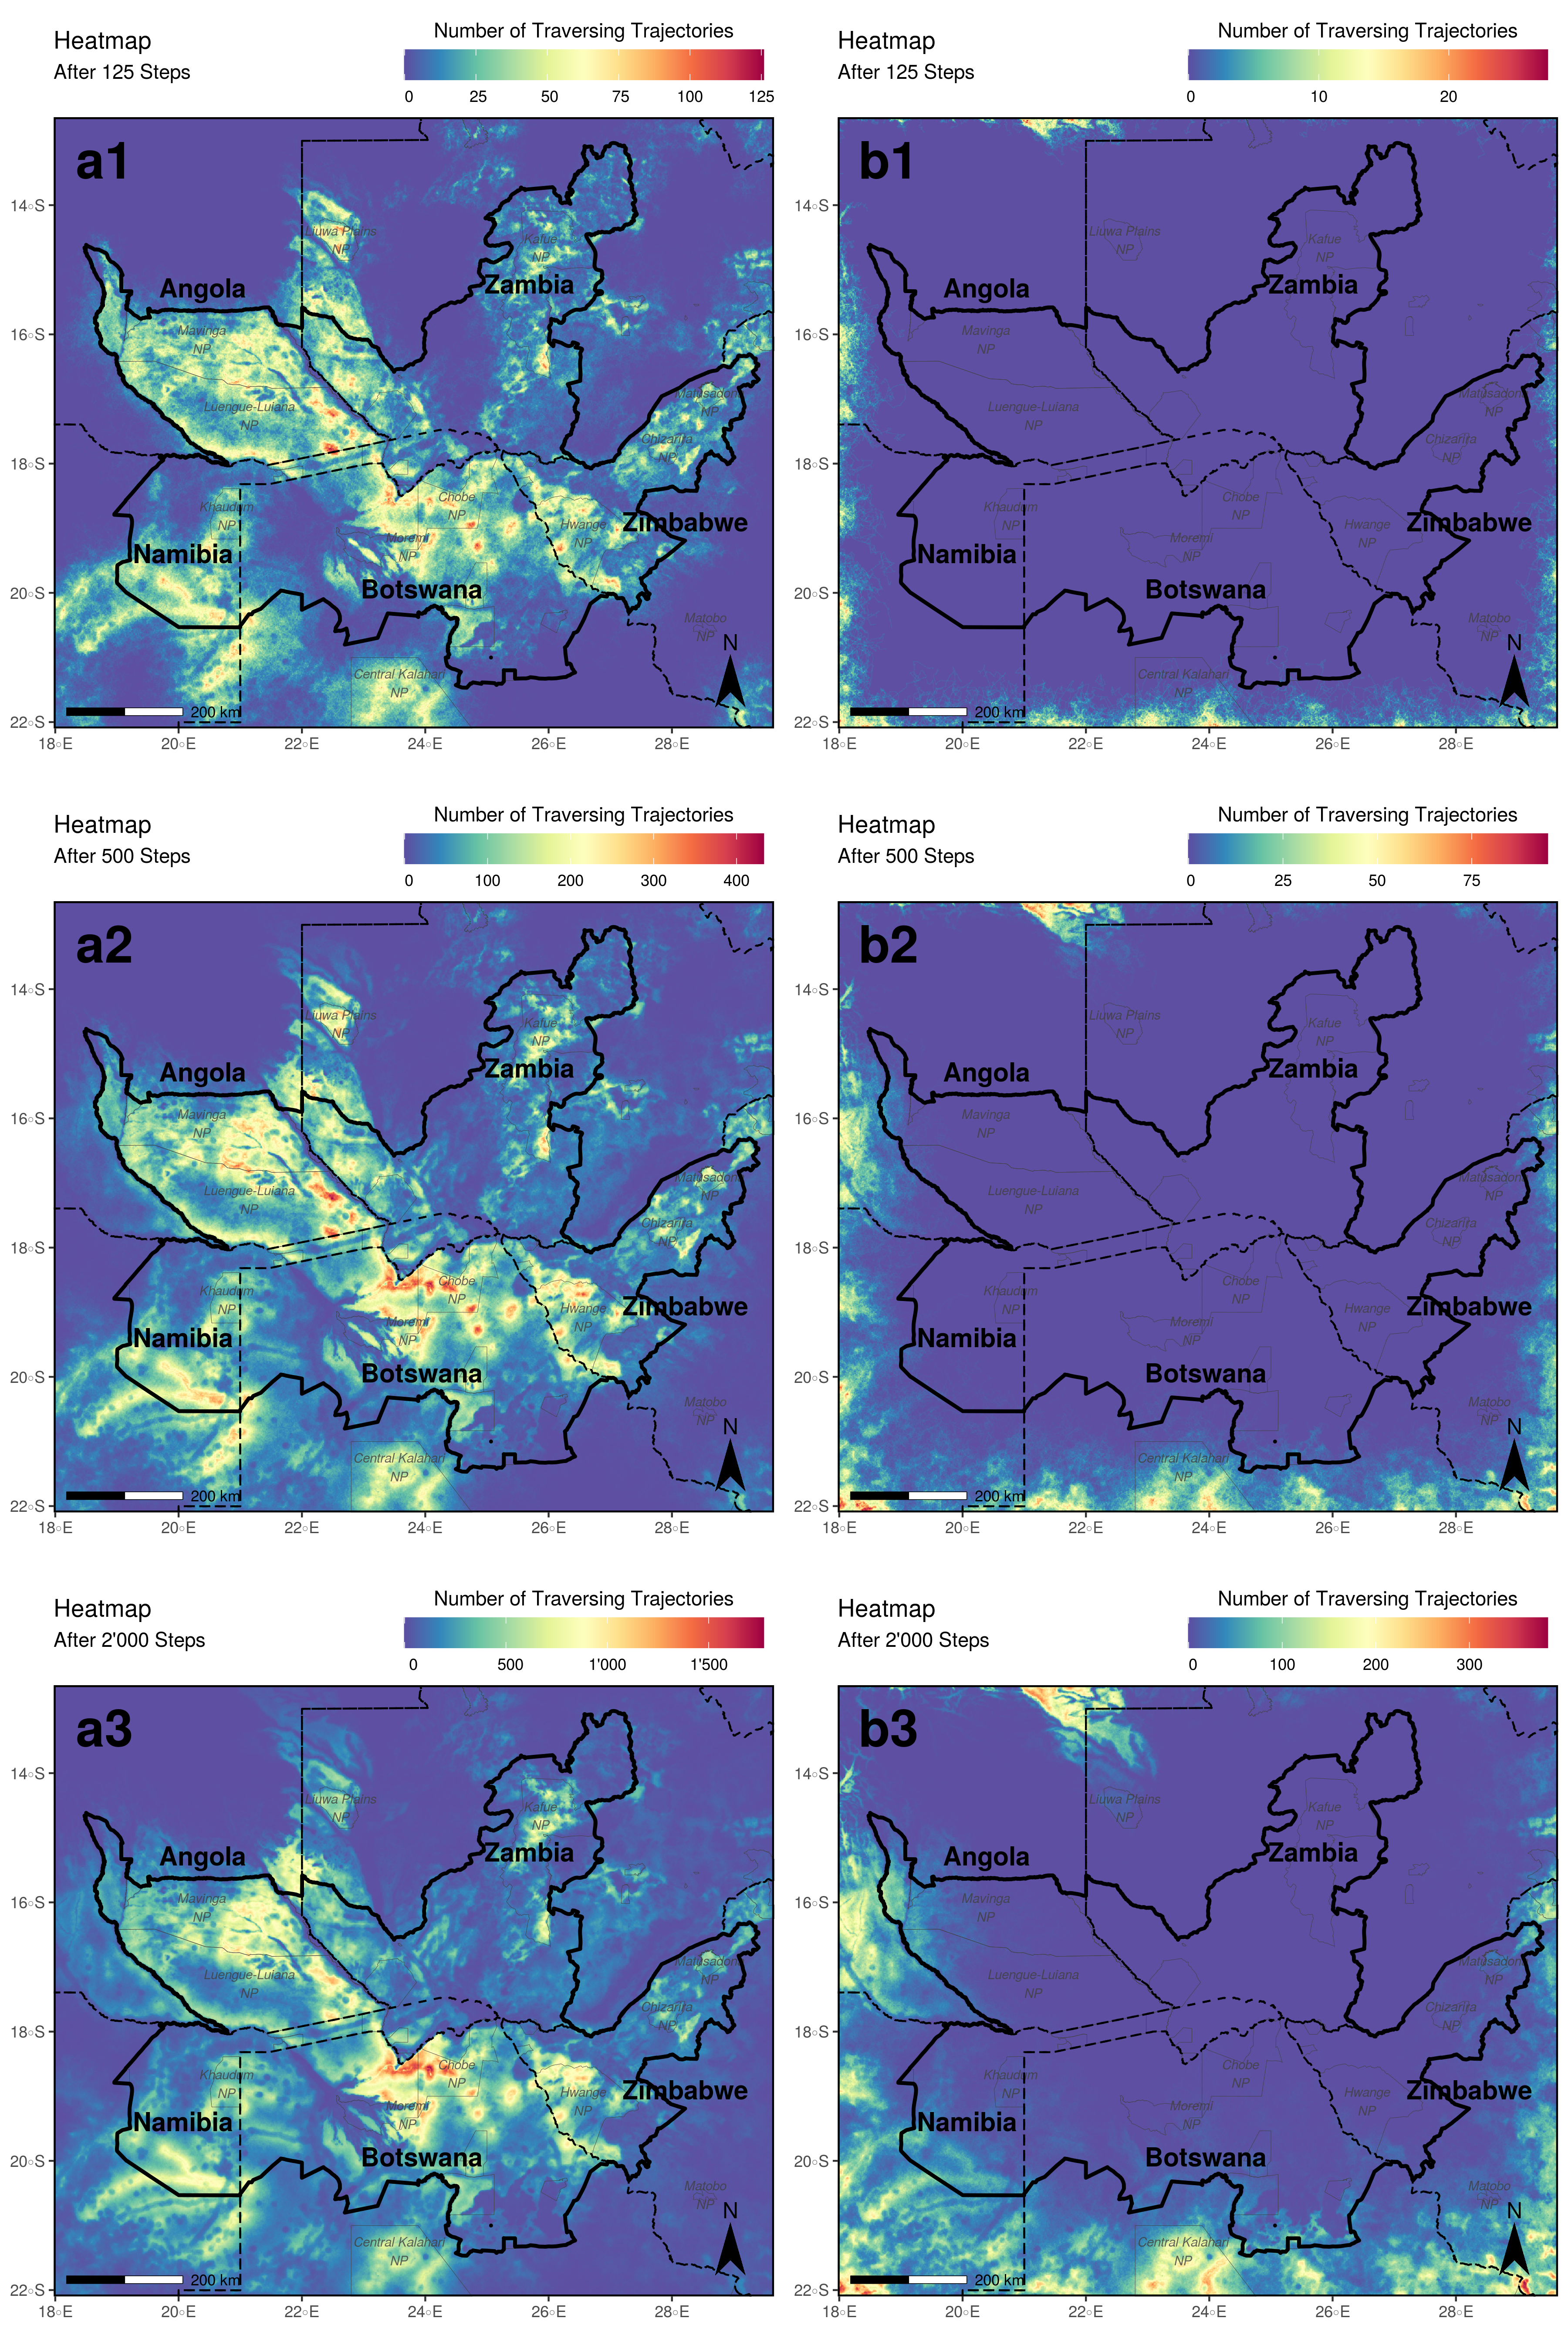
\includegraphics[width = 0.88\textwidth]{99_HeatmapsIndividual.png}
    \caption{Heatmaps produced after 125, 500, and 2000 simulated steps,
    respectively. The left panel (a1, a2, a3) was generated based on simulations
    initiated within the main study area, the right panel (b1, b2, b3) was
    generated based on simulations initiated within the buffer area. To produce
    the heatmap presented in the main text, we summed up values from maps a3 and
    b3.}
    \label{Trajectories}
  \end{center}
\end{figure}
\restoregeometry

%------------------------------------------------------------------------------
%	Appendix S3: Evolution of Betweenness Maps
%------------------------------------------------------------------------------
\newpage
\newgeometry{left=35mm,right=35mm,top=25mm,bottom=10mm,footskip=0pt}
\section{Evolution of Betweenness}
\begin{figure}[hbtp]
  \begin{center}
    \includegraphics[width = 0.88\textwidth]{99_BetweennessIndividual.png}
    \caption{Maps of betweenness scores produced after 125 (a), 500 (b), and
    2000 (c) simulated steps, respectively. A high betweenness score indicates
    that the respective area is paramount for linking other regions in the study
    area. It therefore highlights movement corridors that provide access to
    various destinations.}
    \label{Trajectories}
  \end{center}
\end{figure}
\restoregeometry

\newpage
\begingroup
\singlespacing
\bibliography{Literatur}
\endgroup

\end{document}
